\documentclass{standalone}
\usepackage{tikz}
\usepackage{pgfplots}
\pgfplotsset{compat=1.10}
\usetikzlibrary{arrows}

\definecolor{plot_orange}{RGB}{230,159,0}
\definecolor{plot_blue}{RGB}{86,180,233}
\definecolor{plot_vermillion}{RGB}{213,94,0}

\begin{document}

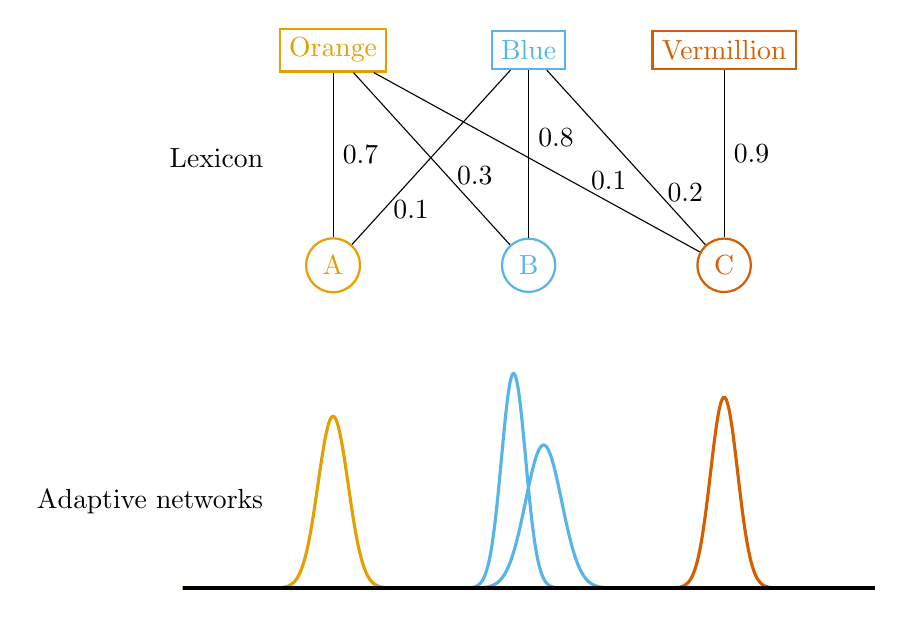
\begin{tikzpicture}

\pgfmathdeclarefunction{gauss}{2}{%
  \pgfmathparse{1/(#2*sqrt(2*pi))*exp(-((x-#1)^2)/(2*#2^2))}%
}

\begin{axis}[no markers, domain=-8:15, samples=500, axis lines=none, width=\textwidth, height=.4\textwidth, clip=false]
\addplot[line width=0.4mm, plot_blue] {gauss(3, 0.4)};
\addplot[line width=0.4mm, plot_blue] {gauss(4, 0.6)};

\addplot[line width=0.4mm, plot_orange] {gauss(-3, 0.5)};

\addplot[line width=0.4mm, plot_vermillion] {gauss(10, 0.45)};

\node[circle, draw, thick, plot_orange] (ca) at (axis cs:-3, 1.5) {A};
\node[circle, draw, thick, plot_blue] (cb) at (axis cs:3.5, 1.5) {B};
\node[circle, draw, thick, plot_vermillion] (cc) at (axis cs:10, 1.5) {C};

\node[rectangle, draw, thick, plot_orange] (la) at (axis cs:-3, 2.5) {Orange};
\node[rectangle, draw, thick, plot_blue] (lb) at (axis cs:3.5, 2.5) {Blue};
\node[rectangle, draw, thick, plot_vermillion] (lc) at (axis cs:10, 2.5) {Vermillion};

\draw (ca) -- node[anchor=west] {0.7} (la);
\draw (ca) -- node[anchor=west, pos=0.2] {0.1} (lb);
\draw (cb) -- node[anchor=west, pos=0.4] {0.3} (la);
\draw (cb) -- node[anchor=west, pos=0.6] {0.8} (lb);
\draw (cc) -- node[anchor=west] {0.9} (lc);
\draw (cc) -- node[anchor=west, pos=0.3] {0.2} (lb);
\draw (cc) -- node[anchor=west, pos=0.4, xshift=1ex] {0.1} (la);

\draw[very thick] (axis cs:-8, 0) -- (axis cs:15, 0);

\node[anchor=east] at (axis cs:-5, 2) {Lexicon};
\node[anchor=east] at (axis cs:-5, 0.4) {Adaptive networks};

\end{axis}

\end{tikzpicture}

\end{document}
